\chapter{Time Distribution}
\label{app:time_distribution}

The project started on December 20th 2013, and was estimated to end on June 13th 2014. The estimated task planning during those 6 months is presented in the section \ref{app:time_tasks}, and a Gantt diagram following that planning is included in section \ref{app:time_gantt}.\\

The critical tasks are the gait optimization and design of the distributed control algorithm, since one cannot foresee the results, and an error in this tasks would suppose an extra workload. Because of that reason, extra time was assigned to those tasks as a buffer to take into accout unexpected outcomes.

\section{Estimated task planning}
\label{app:time_tasks}

\begin{longtable}{|l|p{7cm}|c|c|c|c|}
    \hline
    Code & Task  & Hours & Weeks & Start date & End date  \\ \hline \hline 
    
    1 & \textbf{Study of the state of the art} & 40 & 2 & 20/12/13 & 03/01/14 \\ \hline
    1.1 & Read previous work on the field & 20 & 1 & 20/12/13 & 27/12/13 \\ \hline
    1.2 & Test existing platforms & 20 & 1 & 27/12/13 & 03/01/14 \\ \hline 
    \\ \hline
    
    2 & \textbf{Basic framework development} & 100 & 5 & 03/01/14 & 07/02/14 \\ \hline
    2.1 & Basic digital model & 40 & 2 & 03/01/14 & 17/01/14 \\ \hline
    2.2 & Select and setup simulator & 20 & 1 & 17/01/14 & 24/01/14 \\ \hline
    2.3 & Development of basic control software & 40 & 2 & 24/01/14 & 07/02/14 \\ \hline      
    \\ \hline
    
    3 & \textbf{Optimization of gaits} & 50 & 2.5 & 07/02/14 & 26/02/14 \\ \hline
    3.1 & Algorithm selection & 10 & 0.5 & 07/02/14 & 12/02/14 \\ \hline 
    3.2 & Gait optimization & 40 & 2 & 12/02/14 & 26/02/14 \\ \hline  \\ \hline
  
    4 & \textbf{Distributed control algorithm} & 50 & 2.5 & 26/02/14 & 14/03/14 \\ \hline
    \\ \hline
    
    5 & \textbf{Development of remaining software} & 90 & 4.5 & 14/03/14 & 16/04/14 \\ \hline
    5.1 & Communication-related software & 30 & 1.5 & 14/03/14 & 26/03/14 \\ \hline 
    5.2 & Module distributed controller & 30 & 1.5 & 26/03/14 & 04/04/14 \\ \hline 
    5.3 & Test results & 30 & 1.5 & 04/04/14 & 16/04/14 \\ \hline 
    \\ \hline    

    6 & \textbf{Hardware platform development} & 90 & 4.5 & 16/04/14 & 16/05/14 \\ \hline
    6.1 & Design and manufacture PCB & 30 & 1.5 & 16/04/14 & 25/04/14 \\ \hline 
    6.2 & Design and manufacture mechanical module & 40 & 2 & 25/04/14 & 09/05/14 \\ \hline 
    6.3 & Test results with hardware platform & 20 & 1 & 09/05/14 & 16/05/14 \\ \hline 
    \\ \hline   
        
    7 & \textbf{Documentation and Thesis} & 80 & 4 & 16/05/14 & 13/06/14 \\ \hline
     \multicolumn{2}{|r|}{\textbf{Total}} & \textbf{500} & \textbf{25} & \textbf{20/12/13} & \textbf{13/06/14} \\ \hline
    
\end{longtable}

\newpage

%% Gantt diagram %%
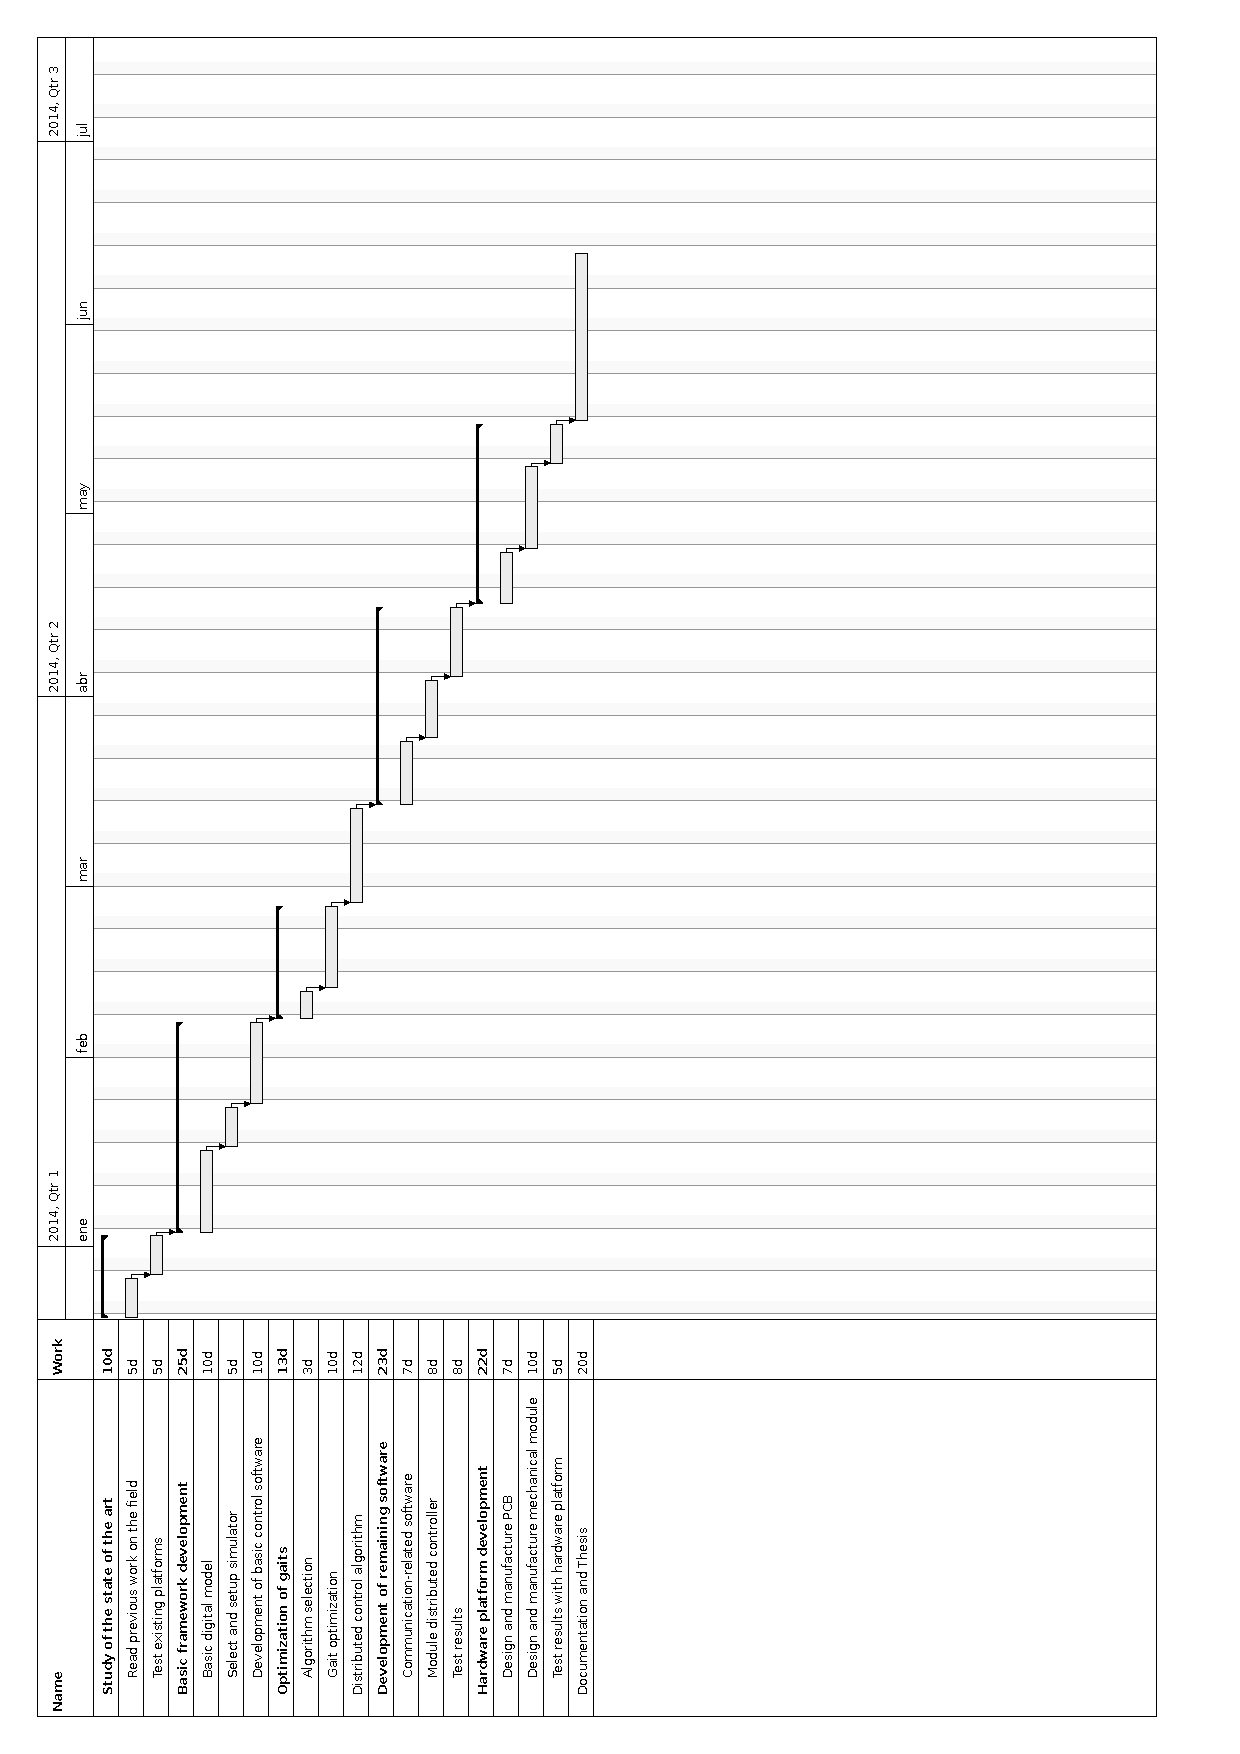
\includepdf[pages=1, scale=0.8, pagecommand=\section{Gantt diagram}\label{app:time_gantt}]{appendices/gantt.pdf}